\documentclass[12pt,ngerman]{scrartcl}

\usepackage[T1]{fontenc}
\usepackage{babel}
\usepackage{graphicx}
\usepackage{xcolor}
\usepackage{tikz}
\usepackage{amsmath}
\usetikzlibrary{shapes}
\pagestyle{empty}

\renewcommand{\familydefault}{\sfdefault}
\begin{document}

\begin{center}
{\footnotesize
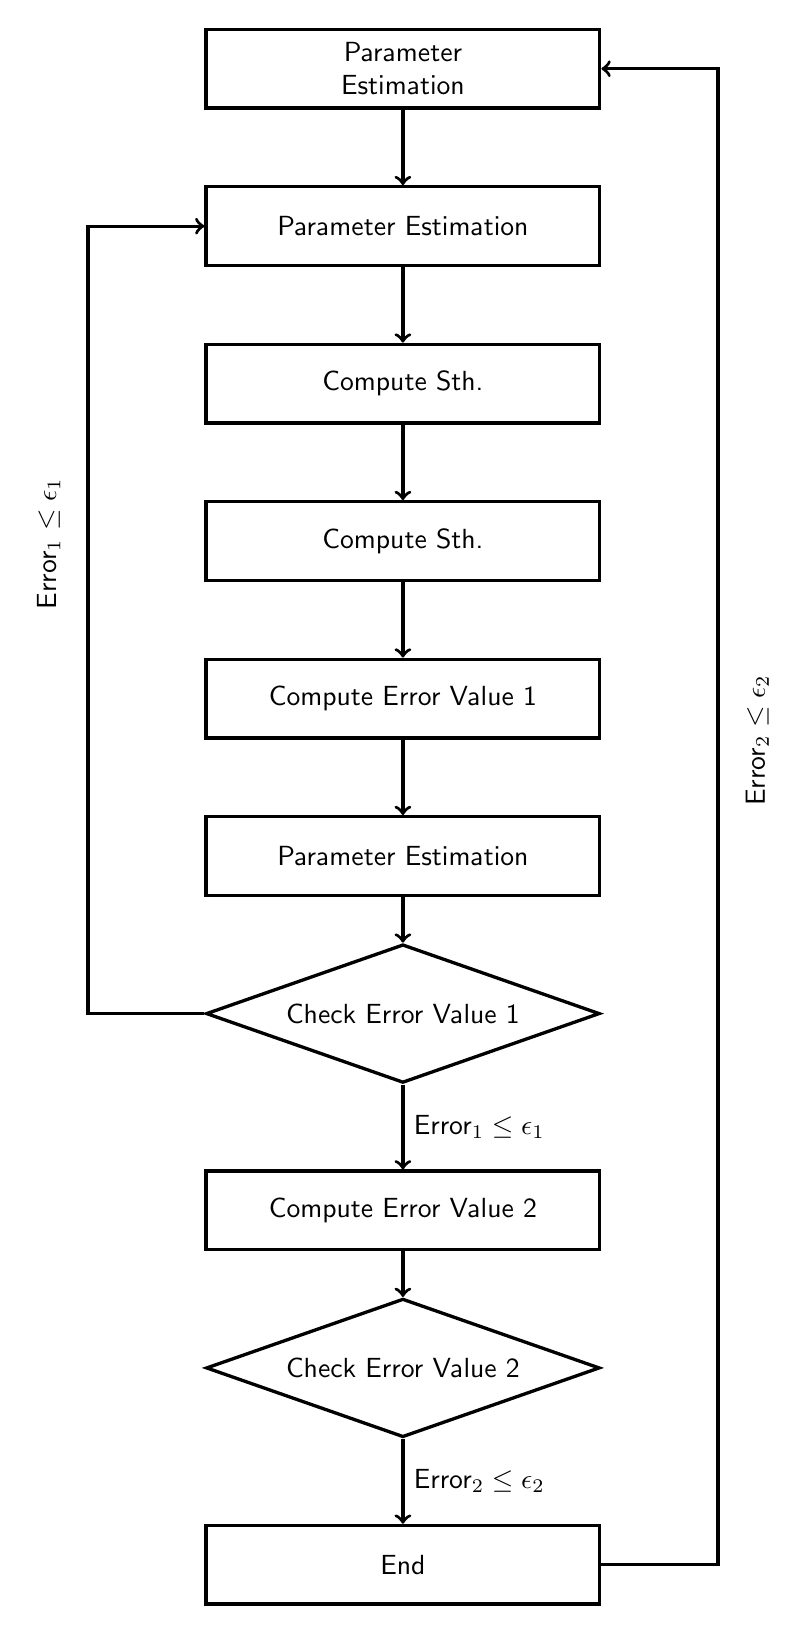
\begin{tikzpicture}
[mybox/.style={rectangle,minimum width=50mm, minimum height=10mm,align=center,draw=black,very thick},
dia/.style={mybox,diamond, aspect=2.5},
]

\node [mybox] (A) at (0,0){Parameter \\ Estimation};
\node [mybox] (B) at (0,-2){Parameter  Estimation};
\node [mybox] (C) at (0,-4){Compute Sth.};
\node [mybox] (D) at (0,-6){Compute Sth.};
\node [mybox] (E) at (0,-8){Compute Error Value 1};
\node [mybox] (F) at (0,-10){{Parameter  Estimation}};
\node [dia] (G) at (0,-12){Check Error Value 1};
\node [mybox] (H) at (0,-14.5){Compute Error Value 2};
\node [dia] (I) at (0,-16.5){Check Error Value 2};
\node [mybox] (J) at (0,-19){End};
\draw[->,very thick] (A) -- (B);
\draw[->,very thick] (B) -- (C);
\draw[->,very thick] (C) -- (D);
\draw[->,very thick] (D) -- (E);
\draw[->,very thick] (E) -- (F);
\draw[->,very thick] (F) -- (G);
\draw[->,very thick] (G) -- (H) node[midway,sloped,right,rotate=90]{\(\text{Error}_1 \leq \epsilon_1\)};
\draw[->,very thick] (H) -- (I);
\draw[->,very thick] (I) -- (J) node[midway,sloped,right,rotate=90]{\(\text{Error}_2 \leq \epsilon_2\)};

\draw[->,very thick] (J) -- (4,-19) -- (4,0) node[midway,yshift=-0.5cm,right,sloped,rotate=0]{\(\text{Error}_2 \leq \epsilon_2\)} -- (A); 
\draw[->,very thick] (G) -- (-4,-12) -- (-4,-2) node[midway,yshift=0.5cm,right,sloped,rotate=0]{\(\text{Error}_1 \leq \epsilon_1\)} -- (B);
\end{tikzpicture}}
\end{center}

\end{document}